% ============================
% Section: Background
% ============================

% General background information about liver cancer and imaging.
%liver cancer types

%\subsection{Liver Cancer Overview}
%\subsection{PET/CT vs. PET/MR in Liver Cancer Radiotherapy}
Liver cancer is particularly difficult to diagnose and its treatment requires highly precise imaging. It needs accurate tumor delineation and because of its size and location spare healthy liver tissue, and organs at risk (OAR). This means radiologists need accuracy, especially when administering targeted therapies \cite{beaton2019, floridi2022}.

Around the world there is a common concern of cancer incidences. Liver cancer, in particular, ranks as the sixth most common diagnosed cancer and the third leading cause of cancer-related deaths. In 2020, approximately 905,700 new cases and 830,200 deaths were reported globally \cite{journal_of_hepatology2022}. 


The global burden varies significantly by region, for example, East Asia and sub-Saharan Africa have the largest incidence rate while in the United States liver cancer rates are comparatively lower. Global predictions estimate that this rates will increase by 55\% between 2020 and 2040, potentially leading to 1.4 million new cases and 1.3 million deaths annually by 2040 \cite{journal_of_hepatology2022}.

The American Cancer society projected approximately 41,630 new cases and 29,840 deaths in the United States \cite{cancer_stats2024}. As the year concludes we may expect to see the actual increase in new cases, however there is a historical increasing trend, the United States have seen, between 1975 and 2017, an increase of 228\% incidence and 137\% rise in mortality. Probably driven by a combination of rising risk factors, aging populations, and improved detection. However, despite advancements in imaging and treatment, late diagnoses and limited therapeutic options have contributed to persistently high mortality rates.

Moreover, projections made in 2020 suggest that liver cancer could become the third leading cause of cancer-related deaths in the US by 2030, surpassing breast, prostate, and colorectal cancers \cite{aacr_2030}. This is particularly interesting, since this has already happen globally, the slower growth of cases an mortality in the U.S. suggests that public health efforts are having a meaningful impact, continued advancements in imaging, personalized therapy, and public health interventions are needed to sustain and further improve outcomes.

%\subsection{Why is Liver Cancer Hard to Diagnose?}
The liver is the largest solid organ located in the upper right quadrant of the abdominal cavity, beneath the diaphragm, its roles includes metabolism, detoxification, and digestion. It is partially shielded by the rib cage, making it relatively protected. To better illustrate its position and function figure \ref{fig:liver-relations} shows the abdominal cavity with the liver’s relationship to adjacent organs such as the stomach, diaphragm, and intestines \cite{lecturio2023,ozmen2020}. 

\begin{figure}[H] % H ensures the image is placed exactly here (requires float package)
	\centering
	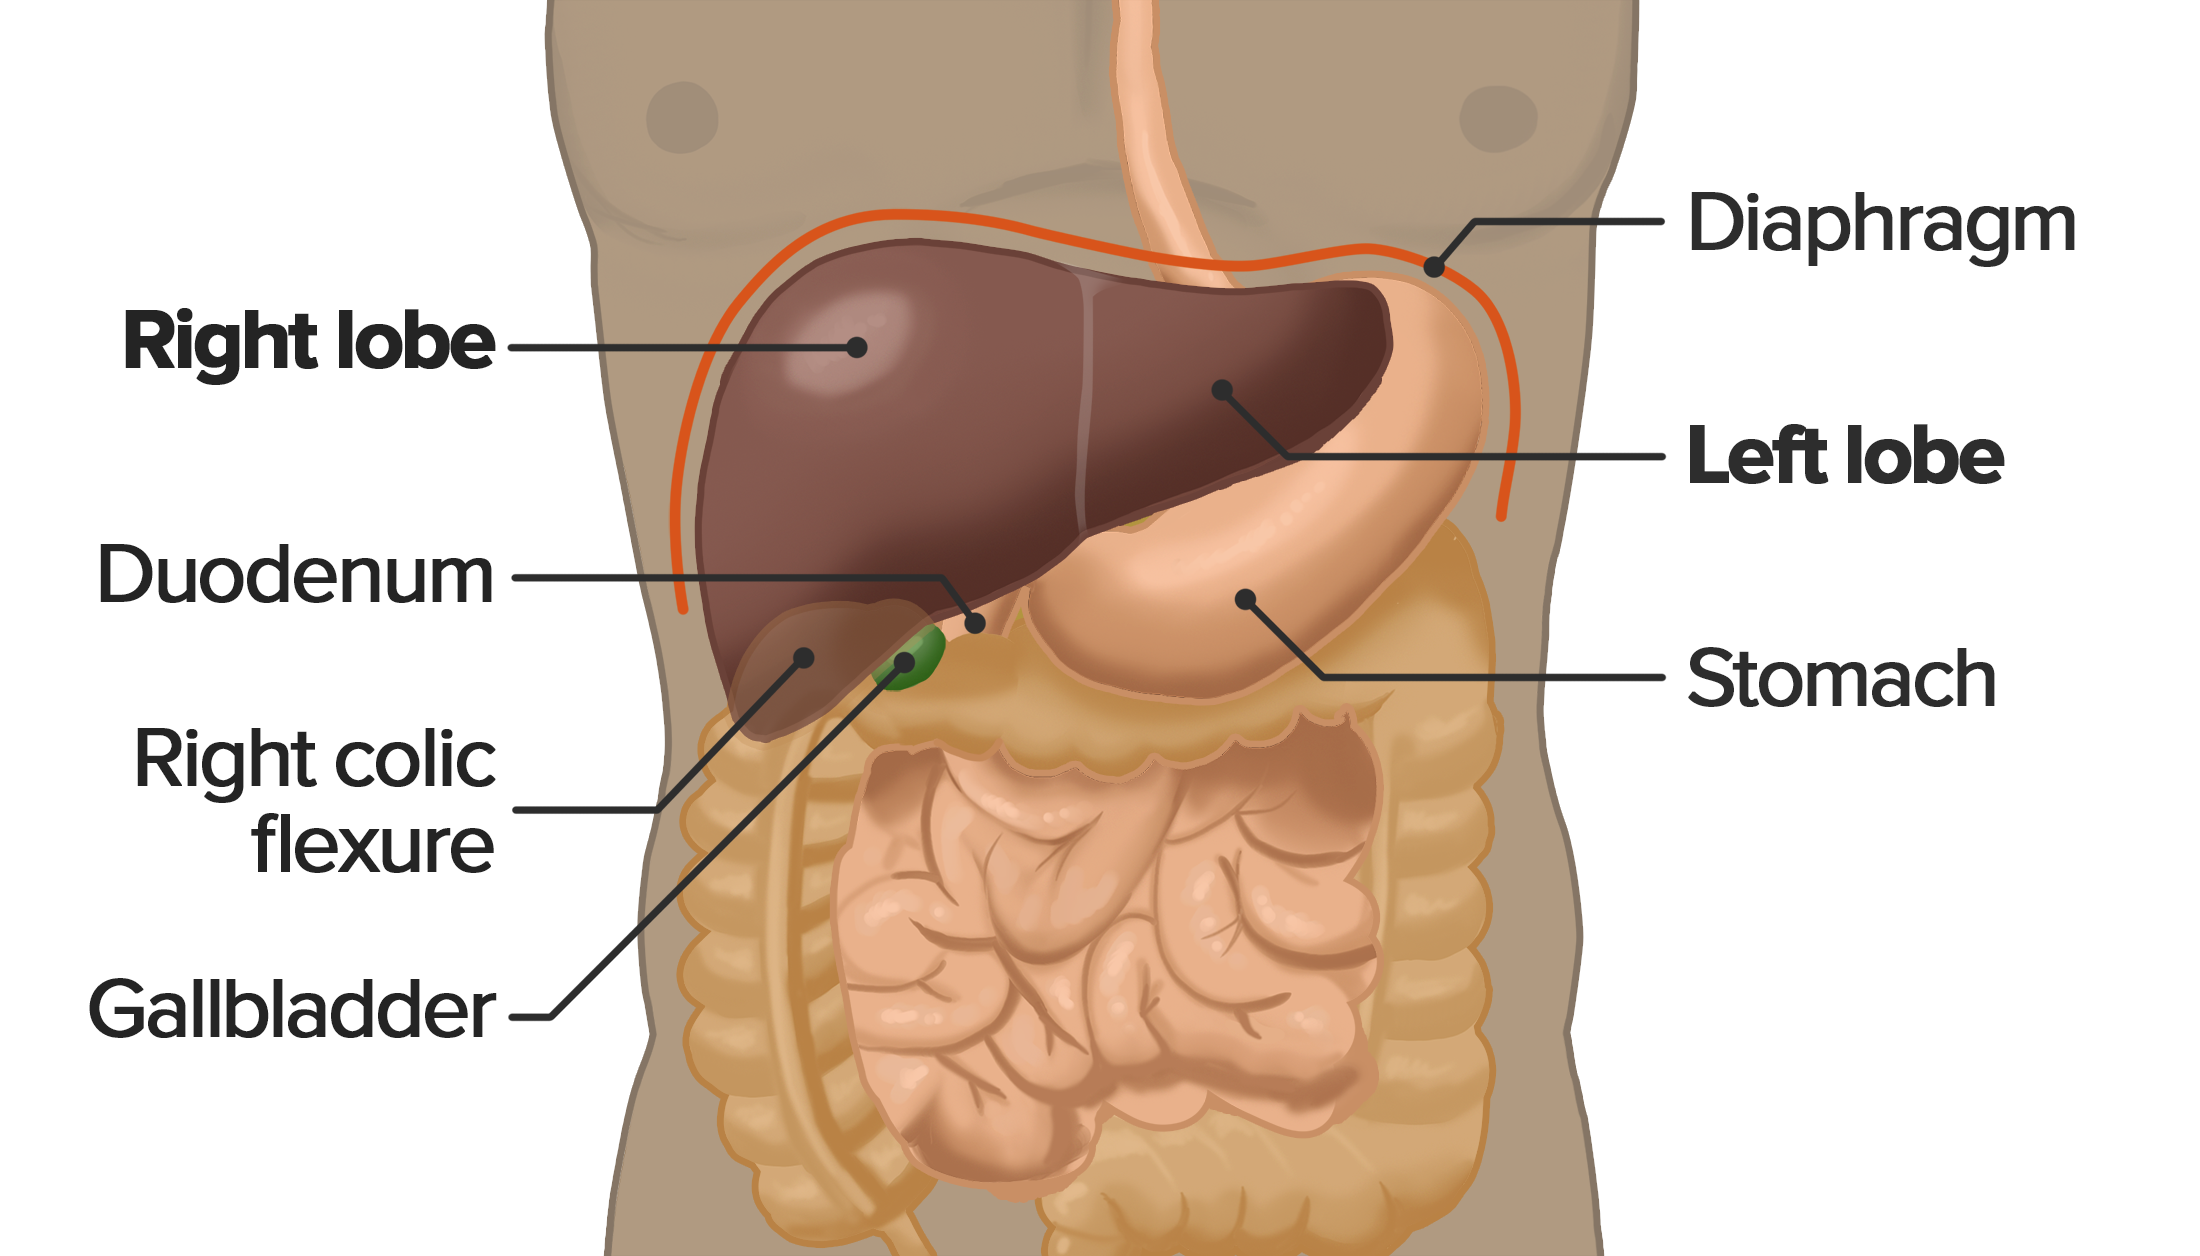
\includegraphics[width=0.5\textwidth]{assets/Liver-relations.png} % Adjust width as needed
	\caption{Anatomical Relations of the Liver}
	\label{fig:liver-relations}
\end{figure}

It has a complex structure, it has two main lobes (right and left), the right lobe is significantly larger, and its main function is metabolic and detoxification processes. The left lobe, is smaller, and it is in charge of production and nutrient metabolism \cite{ozmen2020}.

The liver can be shaped differently between individuals. As shown in Figure \ref{fig:liver-shapes}, the anterior surface of the liver can be classified into four primary shapes.

First, \textbf{Globular Shape (A)} A rounded configuration typically seen in healthy individuals with an average body. Next, \textbf{Conical Shape (B)} Characterized by a narrow right lobe and a smaller left lobe, often observed in elongated torsos. Then, \textbf{Quadrilateral Shape (C)} Exhibits a broader and flatter right lobe with minimal reduction, common in individuals with higher abdominal fat deposition. Finally, \textbf{Rectangular Shape (D)} A flat and wide configuration with a reduced height-to-width ratio \cite{ozmen2020,diagnostics13142371}.


\begin{figure}[ht]
	\centering
	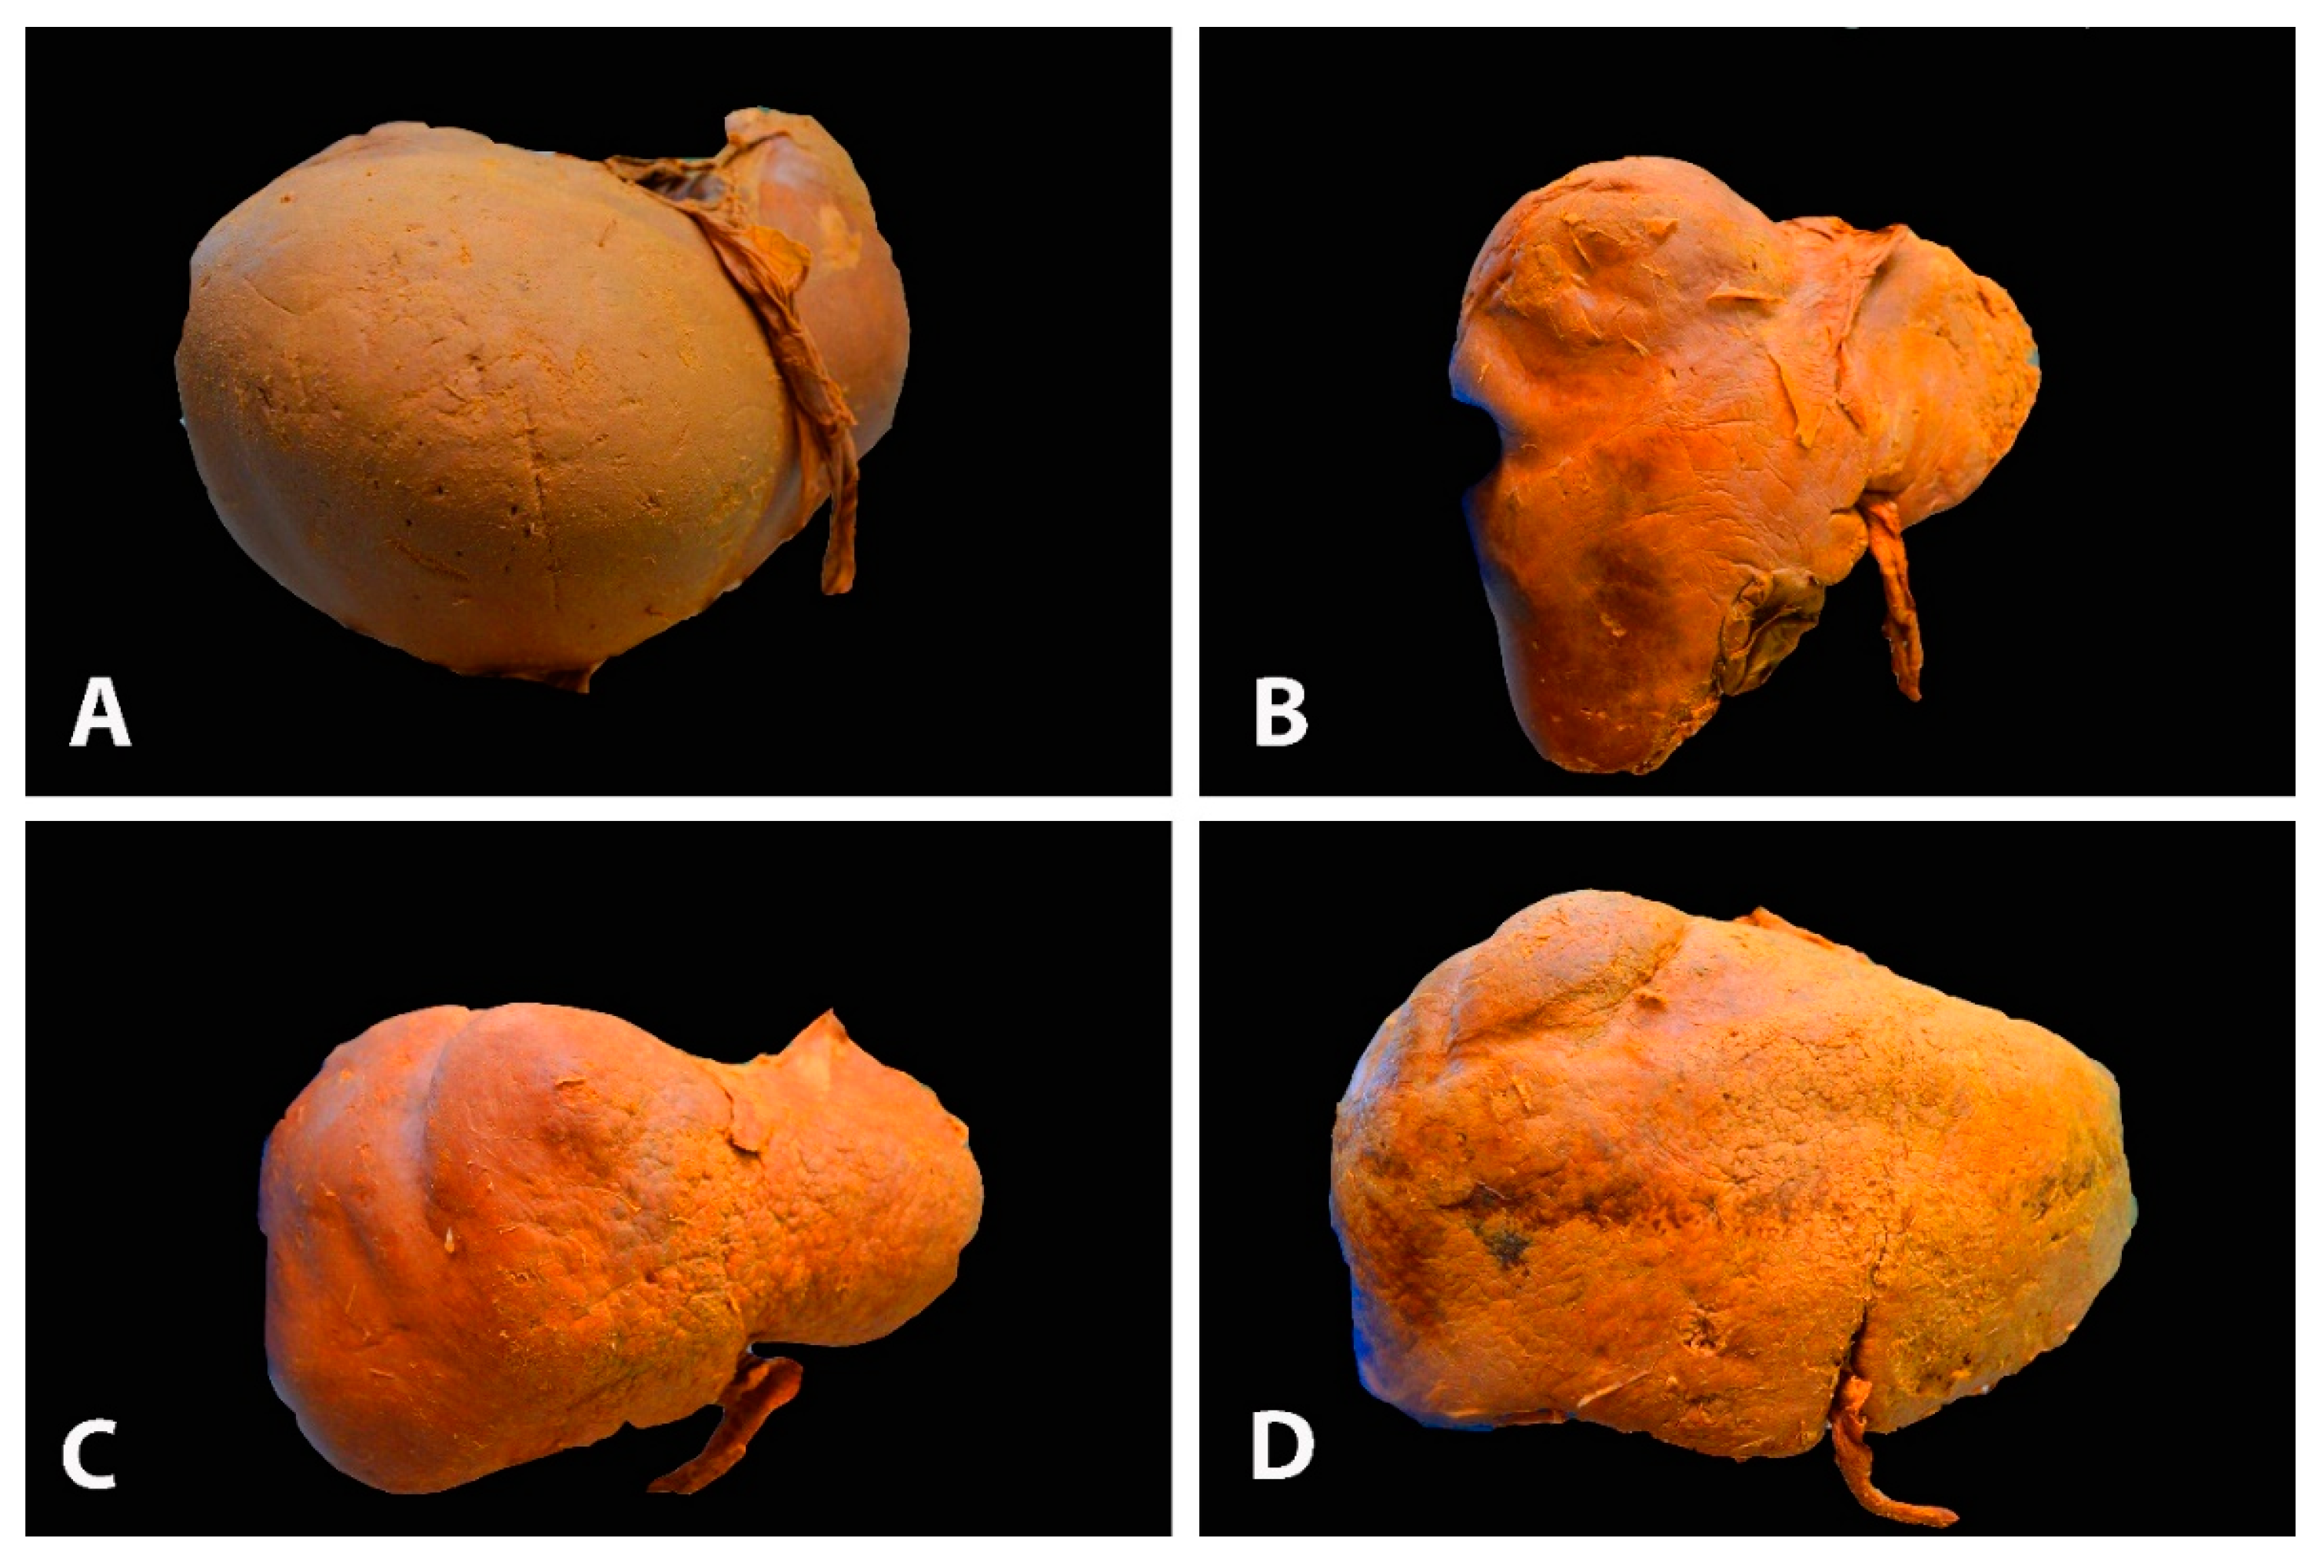
\includegraphics[width=0.45\textwidth]{assets/diagnostics-13-02371-g001.png} % Adjust path to include the relevant figure
	\caption{Anterior surface of the liver classified into four primary shapes: (A) Globular, (B) Conical, (C) Quadrilateral, and (D) Rectangular.}
	\label{fig:liver-shapes}
\end{figure}

Morphological variations directly impact diagnostic accuracy, treatment planning, and therapeutic outcomes. Changes in liver shape due to conditions such as cirrhosis or hepatic steatosis further complicate the diagnostic process, as these conditions alter the liver’s texture and vascular patterns. This can make it challenging to distinguish between benign and malignant lesions on imaging modalities like CT or MRI. Then, the liver is divided into eight segments by functionally, each segment is independent, receiving its own blood supply from a branch of the hepatic artery and portal vein and draining bile through a corresponding biliary branch. This segmention allows precision on diagnostics, surgery and transportation and is depicted on figure \ref{fig:liver-segments-side-by-side} \cite{diagnostics13142371}.

\begin{figure}[H]
	\centering
	\begin{subfigure}[t]{0.25\textwidth}
		\centering
		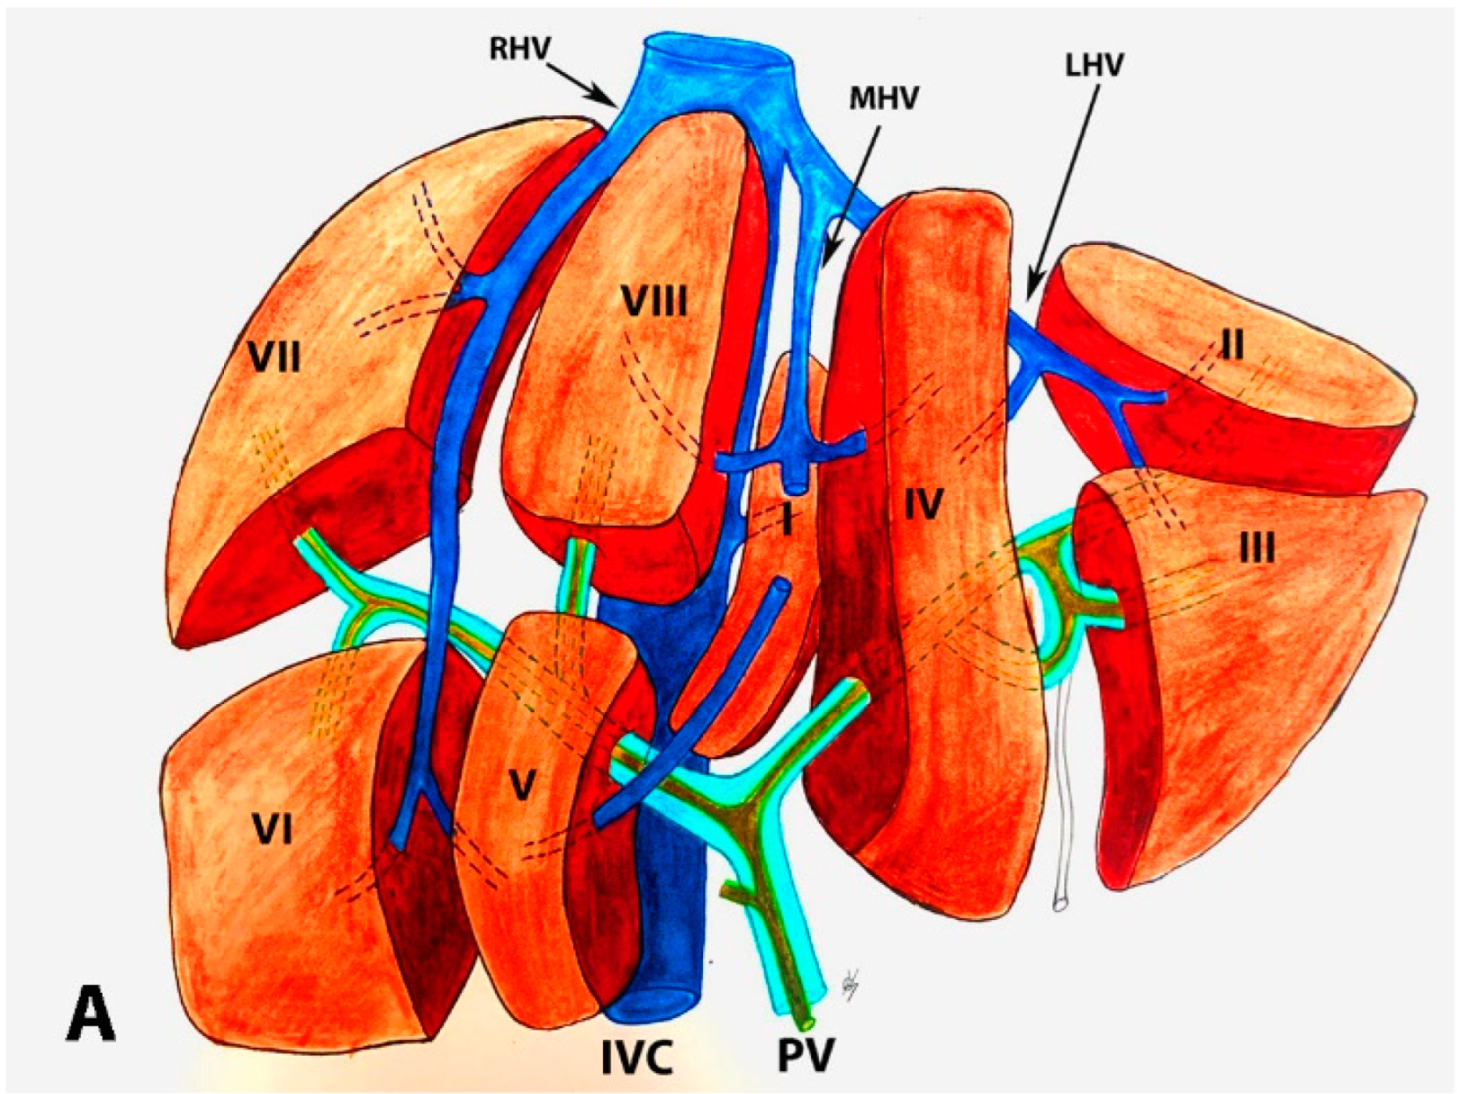
\includegraphics[width=\textwidth]{assets/figure_a.png} % Adjust path if needed
		\caption{}
		\label{fig:figure-a}
	\end{subfigure}
	\hfill
	\begin{subfigure}[t]{0.25\textwidth}
		\centering
		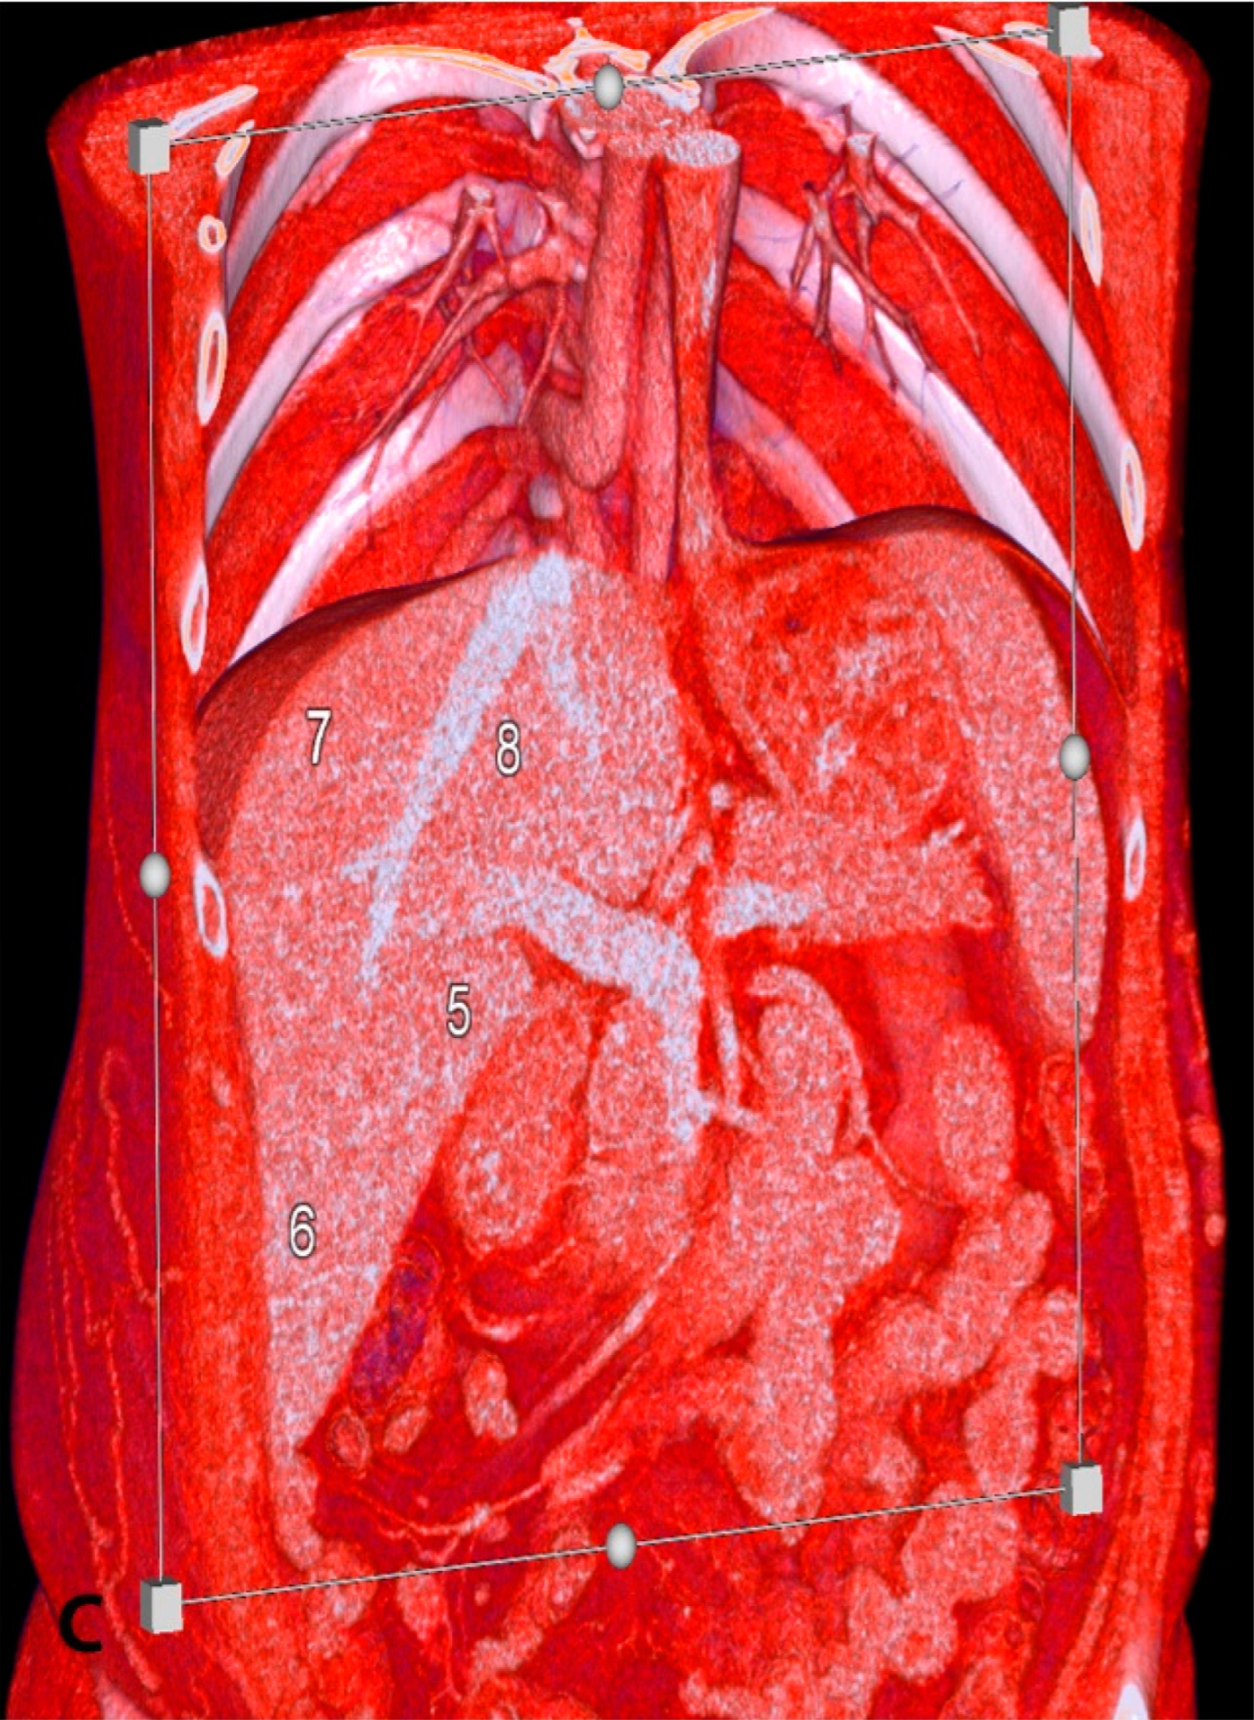
\includegraphics[width=\textwidth]{assets/figure_c.png} % Adjust path if needed
		\caption{}
		\label{fig:figure-c}
	\end{subfigure}
	\caption{Segments of the liver according to Couinaud’s classification: (A) ex vivo appearance; (C) coronal volume-rendered abdominal CT image with annotated right hepatic lobe segments. PV – portal vein; IVC – inferior vena cava.}
	\label{fig:liver-segments-side-by-side}
\end{figure}

The segmented and lobular structure of the liver makes imaging harder. Lesions can be difficult to localize within segments because of overlapping vascular and biliary structures. Small tumors or anomalie in deeper segments like the caudate lobe, which is encircled by other liver regions and  organs, may not be detected. \cite{WJGnet2023,liverMassCharacterization2023}

In radiotherapy, the morphological irregularities, may shift the relative position of tumors within the liver. This necessitates advanced imaging techniques, to precisely map the tumor’s location relative to moving anatomical structures like the diaphragm during the breathing cycle. \cite{luersen2015}

Moreover, the liver’s segmented anatomy and its dual blood supply necessitate careful dosimetric planning to optimize radiotherapy. Variations in lobe size affect the volume of liver tissue exposed to radiation. Additionally, exaggerated organ motion during respiration require adaptive radiotherapy techniques, such as respiratory gating or motion management systems, to ensure accurate dose delivery.\cite{pmc5658876}

Dosimetric planning techniques, such as Intensity-Modulated Radiation Therapy (IMRT) and Volumetric Modulated Arc Therapy (VMAT), take these variations into account by adapting dose distribution to the unique anatomy of each patient, sparing healthy tissues and minimizing complications. \cite{oymak2022}

Diagnosing cancer is a challenge also due to its nature, in particular liver cancer as it presents asymptomatic in early stages, for example hepatocellular carcinoma (HCC) often develops in patients with chronic liver disease or cirrhosis, which can mask early signs of cancer and further complicate detection \cite{quaglia2018,doi:10.1148/radiol.14132362}.

In the other hand there is limitations of standard screening tools, following the HCC example, usually tested with ultrasound and often combined with alpha-fetoprotein (AFP) test. AFP is a serum biomarker commonly used in HCC screening and diagnosis. AFP level increased may suggest underlying pathology, which may be malignant \cite{bialecki2005}.
However, ultrasound and AFP tests have limitations. Ultrasound sensitivity is hindered particularly in patients with obesity or cirrhosis.\cite{floridi2022} Studies have shown that ultrasound can miss more than half of early-stage tumors, while the addition of AFP testing still fails to detect over one-third of early HCC cases \cite{mcmahon2023}.

%\subsubsection{Challenges and Advances in Imaging for Liver Cancer}

Recent years have seen advancements in imaging techniques by combining standard techniques such as CT, MRI, and cone-beam CT (CBCT) to enhance tumor visualization.\cite{floridi2022}.

Imaging the liver is quite difficult due to its location beneath the rib cage, the impact of respiratory motion, and patient-specific factors or comorbilities. The liver’s heterogeneity and its internal complexity further complicate image interpretation. \cite{ferraioli2018}.

Imaging is useful during all stages of treatment. Because of the liver's intricate structure and common comorbidities such cirrhosis, it is important to accurately define tumor borders, determine vascular involvement, and estimate closeness to other tissues \cite{floridi2022}.

The most widely used imaging modality to asses liver cancer is ultrasound (US) due to its accessibility, real-time imaging capability, ability to assess blood flow via Doppler techniques, and because of its non-ionizing nature. But, it is limited by operator skill and sensitivity while detecting small lesions, in early-stage hepatocellular carcinoma (HCC) the smallest detectable lesions typically range from 3 to 5 mm in diameter. \cite{mcmahon2023,ferraioli2018}. 

For instance, small hepatic adenomas, which are benign solid lesions, often remain undetected until they grow larger than 5 cm. Similarly, early-stage intrahepatic cholangiocarcinoma, a bile duct cancer, and small hepatic cysts, which are fluid-filled sacs, are frequently missed unless they become symptomatic or increase in size \cite{tre777}. 

It is hard to diagnose because of two main reasons. The quality of contrast-enhanced ultrasound (CEUS) images heavily depends on the baseline US image, which can be affected by factors such as lesion depth, location (e.g., subdiaphragmatic). Additionally, CEUS typically allows for the evaluation of only one focal liver lesion (FLL) at a time, increasing the risk of overlooking additional small lesions \cite{pmc5588445}.

To overcome this limitations there are hybrid imaging techniques, for example US fused with cone-beam CT (CBCT) or MRI, have significantly enhanced tumor visualization and treatment precision. They together provide better spatial resolution and enhance the vascular anatomy, or increased soft tissue contrast.\cite{floridi2022}.  For instance, US provides excellent spatial resolution for superficial structures, while CBCT and MRI offer high-resolution 3D imaging of deeper tissues, improving the delineation of tumor boundaries \cite{pmc3016679}.

US hybrid approaches also enhance vascular anatomy visualization by combining color Doppler US with contrast-enhanced CT or MRI, particularly useful on planning interventional procedures \cite{frontiers2022}. Moreover, real-time imaging capabilities of US allow for dynamic guidance during procedures. When fused with pre-acquired CBCT or MRI data, its use enhances precision and safety during interventional therapies \cite{rsna2021}.

There is potential to be discovered form hybrid imaging modalities in cancer treatment, that is why now we see increased interest in exploring PET/CT and PET/MR as advanced tools in precision radiotherapy.

Despite significant advancements in imaging technology, further improvements are needed to address intrinsic limitations of CT, MRI, and US in tumor delineation dosimetry, and planing treatment with precision.

CT, offers great spatial resolution but is limited by poor soft tissue contrast and delimitation, it is an irradiating imaging modality and it is suceptible to artifacts caused by metal implants or dental structures \cite{decazes2021}. MRI provides better soft tissue contrast and functional imaging capabilities, yet it lacks the electron density information critical for accurate dose calculations in radiotherapy. Additionally, the extended acquisition times of MRI can introduce motion artifacts, further complicating tumor visualization \cite{floridi2022}.

PET, which provides metabolic and functional data, is often combined with CT or MRI to enhance tumor characterization. However, PET alone suffers from low spatial resolution and partial volume effects, leading to blurred tumor edges and suboptimal delineation of small lesions \cite{yan2024}. These limitations highlight the need for hybrid imaging techniques that leverage the complementary strengths of multiple modalities.

Hybrid approaches such as US/CBCT and CT/MRI fused with US have shown promise in addressing these challenges. For example, CBCT can enhance vascular anatomy visualization in patients with cirrhotic livers, aiding in tumor detection and feeding vessel identification during transarterial treatments \cite{floridi2022}. However, the application of these techniques in radiotherapy remains limited due to technical constraints such as the need for precise attenuation correction and standardized protocols for image registration. Hybrid imaging modalities such as PET/CT and PET/MR are emerging tools for overcoming these barriers, offering improved tumor delineation, dosimetry accuracy, and treatment planning for liver cancer. \cite{knesaurek2018,zhou2021}
